\begin{table}
    \centering
    \caption{性能比较}\label{table:performance}
    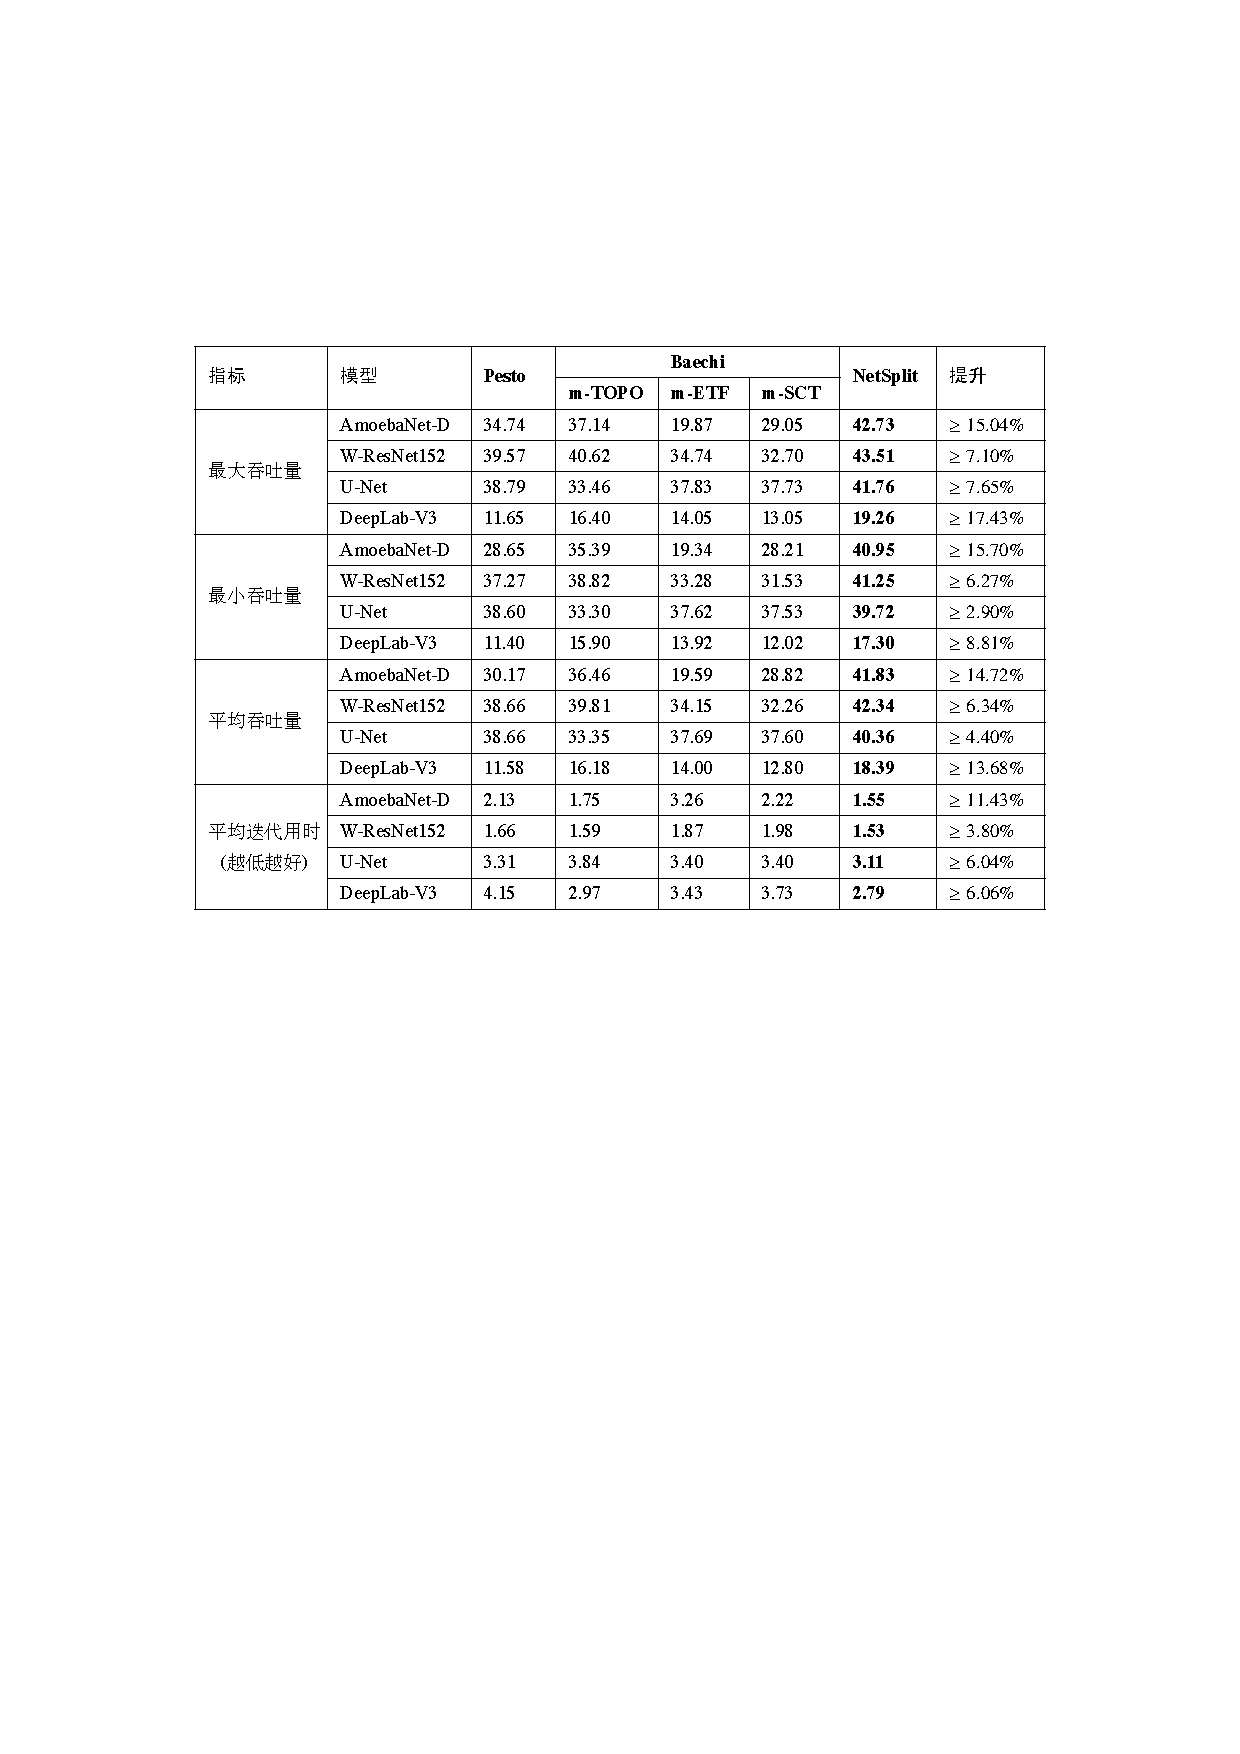
\includegraphics[width=0.98\textwidth]{figure/5-evaluation/performance-table.pdf}
\end{table}

% \begin{table}[h!] % just use this specifier if really needed.
%     \centering
%     \caption{性能比较}\label{table:performance}
%     \tiny
%     \begin{tabular}{ |p{1.8cm} |p{2.0cm} |p{1.0cm} |p{1.3cm} |p{1.1cm} |p{1.1cm} |p{1.2cm} |p{1.4cm}| }
%         \hline
%         \multirow{2}{*}{\textbf{指标}} & \multirow{2}{*}{\textbf{模型}} & \multirow{2}{*}{\textbf{Pesto}} & \multicolumn{3}{c|}{\textbf{Baechi}} & \multirow{2}{*}{\textbf{NetSplit}}  & \multirow{2}{*}{\textbf{提升}}  \\ 
%         \cline{4-6} 
%         & & &\textbf{m-TOPO} & \textbf{m-ETF} & \textbf{m-SCT} & &\\  
%         \hline
%         \multirow{4}{*}{最大吞吐量} & AmoebaNet-D  &  34.74 & 37.14 & 19.87 & 29.05 & \textbf{42.73} & $\ge 15.04\%$ \\
%                                   \cline{2-8}
%                                   & W-ResNet152 &39.57 & 40.62 & 34.74 & 32.70 & \textbf{43.51} & $\ge 7.10\%$ \\
%                                   \cline{2-8}
%                                   & U-Net          &38.79 & 33.46 & 37.83 & 37.73 & \textbf{41.76} & $\ge 7.65\%$ \\
%                                   \cline{2-8}
%                                   & DeepLab-V3    &11.65 & 16.40 & 14.05 & 13.05 & \textbf{19.26} & $\ge 17.43\%$ \\
%         \hline
%         \multirow{4}{*}{最小吞吐量} & AmoebaNet-D  &  28.65 & 35.39 & 19.34 & 28.21 & \textbf{40.95} & $\ge 15.70\%$ \\
%                                   \cline{2-8}
%                                   & W-ResNet152 &37.27 & 38.82 & 33.28 & 31.53 & \textbf{41.25} & $\ge 6.27\%$ \\
%                                   \cline{2-8}
%                                   & U-Net          &38.60 & 33.30 & 37.62 & 37.53 & \textbf{39.72} & $\ge 2.90\%$ \\
%                                   \cline{2-8}
%                                   & DeepLab-V3    &11.40 & 15.90 & 13.92 & 12.02 & \textbf{17.30} & $\ge 8.81\%$ \\
%         \hline
%         \multirow{4}{*}{平均吞吐量} & AmoebaNet-D  & 30.17 & 36.46 & 19.59 & 28.82 & \textbf{41.83} & $\ge 14.72\%$ \\
%                                   \cline{2-8}
%                                   & W-ResNet152 &38.66 & 39.81 & 34.15 & 32.26 & \textbf{42.34} & $\ge 6.34\%$ \\
%                                   \cline{2-8}
%                                   & U-Net         &38.66 & 33.35 & 37.69 & 37.60 & \textbf{40.36} & $\ge 4.40\%$ \\
%                                   \cline{2-8}
%                                   & DeepLab-V3     &11.58 & 16.18 & 14.00 & 12.80 & \textbf{18.39} & $\ge 13.68\%$ \\
%         \hline
%         \multirow{4}{*}{\makecell{平均迭代用时\\(越低越好)}} & AmoebaNet-D    &2.13& 1.75& 3.26& 2.22&  \textbf{1.55} &  $\ge 11.43\%$\\
%                                                          \cline{2-8}
%                                                         & W-ResNet152 & 1.66& 1.59& 1.87& 1.98& \textbf{1.53} & $\ge 3.80\%$\\
%                                                          \cline{2-8}
%                                                         & U-Net          & 3.31& 3.84& 3.40& 3.40& \textbf{3.11} & $\ge 6.04\%$ \\
%                                                          \cline{2-8}
%                                                         & DeepLab-V3     & 4.15& 2.97& 3.43& 3.73& \textbf{2.79} & $\ge 6.06\%$\\
%         \hline
%     \end{tabular}
% \end{table}


% \begin{table}[h!] % just use this specifier if really needed.
%     \centering
%     \caption{性能比较}\label{table:performance}
%     \tiny
%     \begin{tabularx}{\linewidth}{ p{1.4cm} p{1.7cm} p{1.4cm} p{1.4cm} p{1.4cm} p{1.4cm} p{1.4cm} p{1.2cm}}
%         \toprule 
%         \multirow{2}{*}{\textbf{指标}} & \multirow{2}{*}{\textbf{模型}} & \multirow{2}{*}{\textbf{Pesto}} & \multicolumn{3}{c}{\textbf{Baechi}} & \multirow{2}{*}{\textbf{NetSplit}}  & \multirow{2}{*}{提升}\\ 
%         \cmidrule{4-6} 
%         & & &\textbf{m-TOPO} & \textbf{m-ETF} & \textbf{m-SCT} & \\  
%         \midrule
%         \multirow{4}{*}{最大吞吐量} & AmoebaNet-D    & & & & & & \\
%                                   \cmidrule{2-8}
%                                   & W-ResNet152 & & & & & & \\
%                                   \cmidrule{2-8}
%                                   & U-Net          & & & & & & \\
%                                   \cmidrule{2-8}
%                                   & DeepLab-V3     & & & & & & \\
%         \midrule
%         \multirow{4}{*}{最小吞吐量} & AmoebaNet-D    & & & & & & \\
%                                   \cmidrule{2-8}
%                                   & W-ResNet152 & & & & & & \\
%                                   \cmidrule{2-8}
%                                   & U-Net          & & & & & & \\
%                                   \cmidrule{2-8}
%                                   & DeepLab-V3     & & & & & & \\
%         \midrule
%         \multirow{4}{*}{平均吞吐量} & AmoebaNet-D    & & & & & & \\
%                                   \cmidrule{2-8}
%                                   & W-ResNet152 & & & & & & \\
%                                   \cmidrule{2-8}
%                                   & U-Net          & & & & & & \\
%                                   \cmidrule{2-8}
%                                   & DeepLab-V3     & & & & & & \\
%         \midrule
%         \multirow{4}{*}{平均迭代用时} & AmoebaNet-D    & & & & & & \\
%                                     \cmidrule{2-8}
%                                     & W-ResNet152 & & & & & & \\
%                                     \cmidrule{2-8}
%                                     & U-Net          & & & & & & \\
%                                     \cmidrule{2-8}
%                                     & DeepLab-V3     & & & & & & \\
%         \bottomrule
%     \end{tabularx}
% \end{table}